\chapter{Implementation}
\label{ch:implementation}


In this chapter, details of the implementation practical part of the study is discussed. The architecture, modules, development tools, installation, and configurations of such part are the main role of this chapter.  
 
\section {Architecture}
The design of the architecture was planned based on the Input-Process-Output Model. It can be also considered as a black-box solution where the solution processes the input, then it delivers the output once it is ready. follows is the discussion of those 3 phases, described in Figure \ref{Fig:Architecture} : 
 \begin{figure}[H]
	\begin{center}
		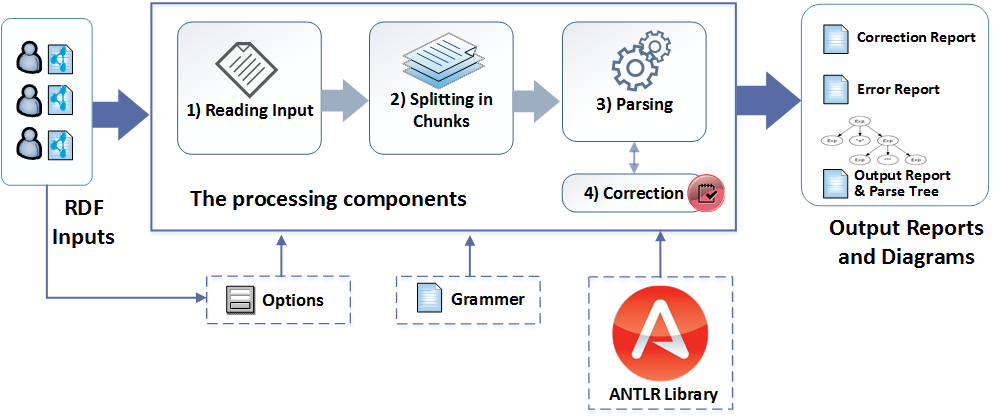
\includegraphics[scale=0.5]{images/Architecture}
		\setlength\belowcaptionskip{-7mm}
		\caption{The proposed solution architecture}
		\label{Fig:Architecture}
	\end{center}
\end{figure}

 \begin{itemize}
 \item \textbf {Input}: It is the role of the user to supply an RDF text with certain options, such as 1) enabling/disabling of the error correction, 2) showing an error report of JSON \footnote{\href{https://www.json.org/}{JSON}} or text format, and 3) concealing/showing up the parse tree.
\item \textbf{Process}: starts with preparing the input ready to be parsing in the following flow: 1)it reads the input, 2) slices it into smaller pieces if needed, 3) parses the input itself or each slice, and 4) corrects some detected syntax errors. This phase was built based on a predefined grammar, it requires ANTLR library for parsing, and some options from the user to activate/deactive some features of the solution.   
\item \textbf{Output}: provides the reports after processing the input, including 1) an errors report to announce the detected syntax errors, 2) a correction report to report the recovered syntax errors, and 3) an output file after healing some of the detected syntax errors, and 4) a frame contains the parse tree. Both of the correction report and the output file need the enabling of the error correction feature to be generated. 
\end{itemize}



\section {Modules} 

	\begin{figure}[ht]
	\begin{center}
		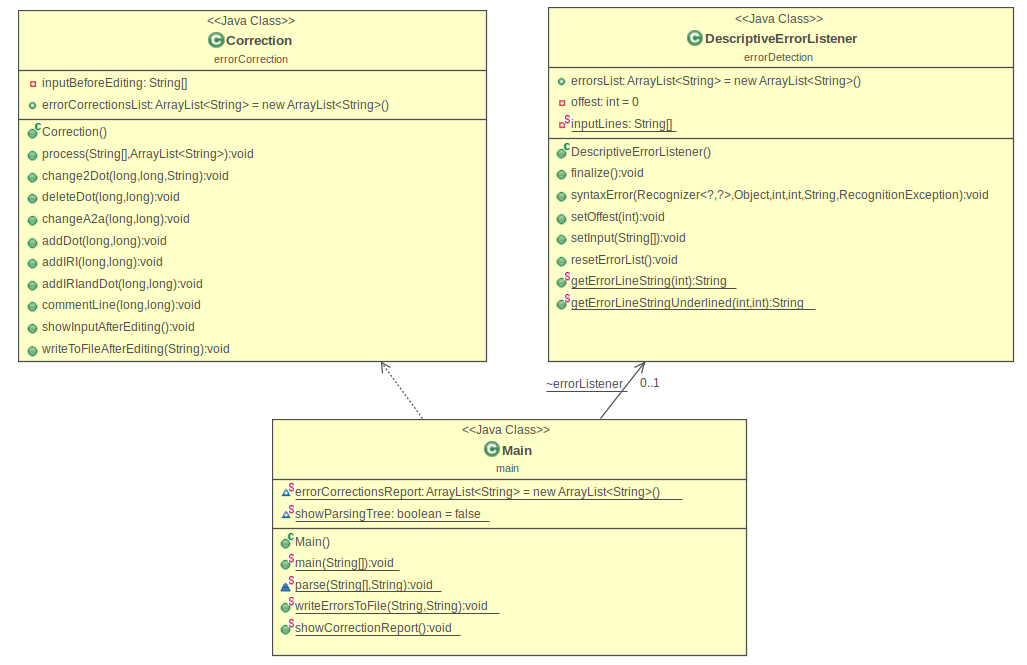
\includegraphics[scale=0.5,angle=0]{images/modules.png}
				\setlength\belowcaptionskip{-7mm}
		\caption{UML diagram for the major modules in the proposed solution}
		\label{Fig:UML}
	\end{center}
\end{figure}

After briefing the proposed solution architecture, It is the time to cover it in more details by shedding light onto those modules which represent the pillars of such solution. {Figure \ref{Fig:UML}} establishes a UML diagram for the most significant modules in this solution, represented into 3 modules: Main, Error Detection, and Error Correction. The following text discusses those modules plus Core module. It is worth to be noted that Core module is not shown in {figure \ref{Fig:UML}} to facilitate the understanding of the main modules, otherwise it would be complex, furthermore, Core is automatically generated module by ANTLR based on the given grammar, thereby few changes were coded in the module:  
 \begin{enumerate}[]
 \item \textbf {Core}: is automatically generated by ANTLR based on the grammar defined appendix \ref{ch:appendix}. It encloses the parsing classes such as Parser, Lexer, Error Collector, Parse Tree Creator.   
\item \textbf{Errors Detection}: listens to the generated error messages by the parser. conventionally, while parsing if the parser detects syntax errors it sends a detail of the error to an error listener if one was defined. This module translates the list of errors were collected by the error listener into a valuable information about the error, such as an error expressive message to express the actual found error, an error location, identified by line and column numbers, and sometimes the actual line text where the parser has disclosed that error.
\item \textbf {Error Correction}: corrects those syntax errors which have only a well-know solution, this module was codded. The error message plays an important role to identify whether it can such error can be corrected or not. A global list stores all detected syntax errors messages and their location in the input (line number and column number) and this modules has predefined messages. if any of the detected error message matches any of the predefined messages, then such error can be healed and recovered.
\item \textbf{Main}: is the executive part which combines input, output, and processing components. It receives the input text, and if it is large (for example, more than 1 million lines), it is segmented into one or more chunks based on its size. Each chunk is handled separately in regards of parsing, error detection, as well as in error correction.

\end{enumerate} 

%TODO:check here how to adjust the vertical space 
\vspace{-5mm}

\section{Real-World Use Cases}
In this section, some of use cases tackled in this study to detect syntax errors in RDF input and  the method of error correction of some of those detected syntax error will be exposed. As a start, let's begin with a Turtle example which has no syntax errors, then some syntax errors can be introduced to show the process of handling them. 
	\vspace{5mm} %5mm vertical space

Listing \ref{lst:turtleExample} shows a Turtle example without syntax errors. First 4 lines are directives or prefixes declaration, rest of lines are triples.  For that reason, our grammar in appendix \ref{ch:appendix} was initialized with the topmost node \textbf{start}  which describes the coming rules by zero or more  \textbf{statement}(s). In addition, each \textbf{statement} is either a directive or a triple as it is represent in \ref{lst:startingRules}.

\begin{lstlisting}[label=lst:startingRules, caption={Starting rules in the grammar file}] 
start
: statement*  EOF
;
statement
: directive
| triples '.'
\end{lstlisting}

\begin{lstlisting}[label=lst:turtleExample, numbers=left, caption={RDF example in Turtle serialization format}]
<@\textcolor{blue}{@prefix}@>  <@\textcolor{red}{rdf}@>: <@\textcolor{orange}{<http://www.w3.org/1999/02/22-rdf-syntax-ns#>}@> .
<@\textcolor{blue}{@prefix}@>  <@\textcolor{red}{rdfs}@>:  <@\textcolor{orange}{<http://www.w3.org/2000/01/rdf-schema#>}@> .
<@\textcolor{blue}{@prefix}@>  <@\textcolor{red}{ex}@>:  <@\textcolor{orange}{<http://example.org/>}@> .
<@\textcolor{blue}{@prefix}@>  <@\textcolor{red}{zoo}@>:   <@\textcolor{orange}{<http://example.org/zoo/> }@> .
<@\textcolor{red}{ex}@>:dog1  <@\textcolor{red}{rdf}@>:type  <@\textcolor{red}{ex}@>:animal .
<@\textcolor{red}{ex}@>:cat1  <@\textcolor{red}{rdf}@>:type  <@\textcolor{red}{ex}@>:cat ;
         <@\textcolor{red}{rdfs}@>:label   <@\textcolor{green}{"Lusi"@en}@> .
<@\textcolor{red}{ex}@>:cat  <@\textcolor{red}{rdfs}@>:subClassOf  <@\textcolor{red}{ex}@>:animal .
<@\textcolor{red}{zoo}@>:host  <@\textcolor{red}{rdfs}@>:range  <@\textcolor{red}{ex}@>:animal .
<@\textcolor{red}{ex}@>:zoo1  <@\textcolor{red}{zoo}@>:host  <@\textcolor{red}{ex}@>:cat2 .
\end{lstlisting}



\begin{figure}

	\begin{subfigure}[]{}
		\centering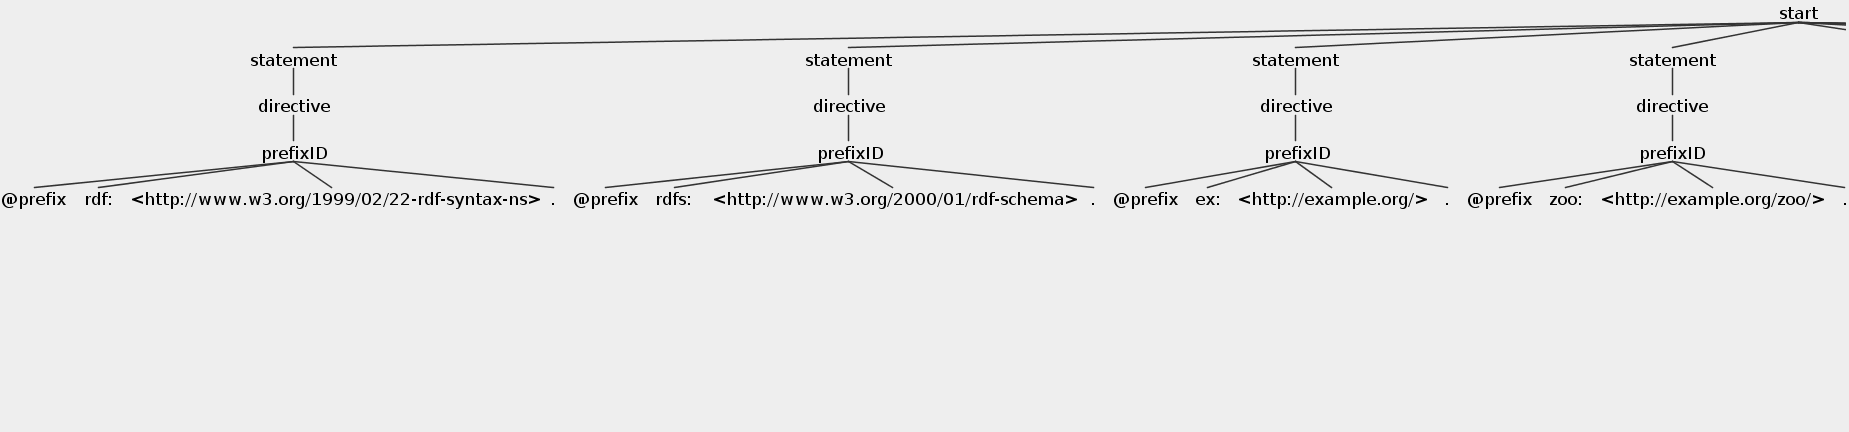
\includegraphics[width=1\linewidth]{images/parseTreeAllLeft.png}
	\end{subfigure}     
		\centering
	\begin{subfigure}[]{}
		\centering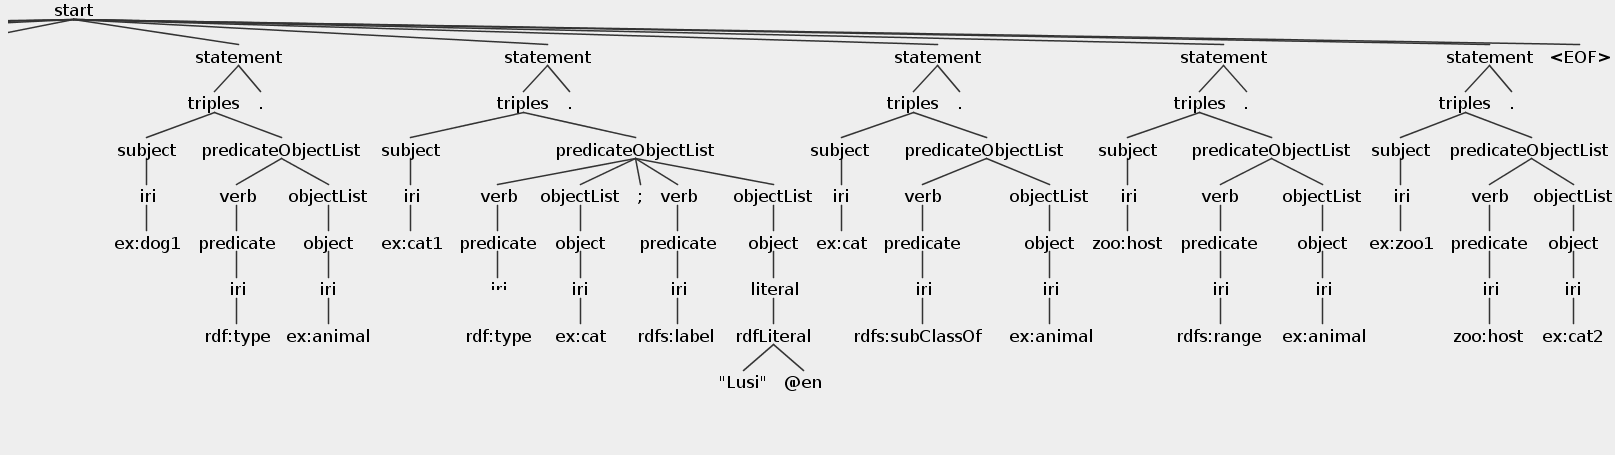
\includegraphics[width=1\linewidth]{images/parseTreeAlRight.png}
		\label{fig:rightSideParseTree}
	\end{subfigure}
	\caption{The parse tree view of listing \ref{lst:turtleExample}. (a) shows the left-side tree and (b) is the right-side tree. Both (a) and (b) are siblings of the parent node \textbf{start} in the parse tree  }
	\label{Fig:parseTreeTAll}
\end{figure}

After showing up a part of grammar rules and views of the parse tree, some of real cases of handling error detection and error recovery will be presented:
\begin{enumerate}
    \item \textbf{Missing a dot at the end of a triple:} in Turtle syntax, a triple must ends with a dot. In listing \ref{lst:missingDotEx}, the head rule \textbf{statement} as it was previously described, can be either directives or triples (ends with a dot). Equally important the last line which shows that triples without a dot can be also a sub-goal of this rule. This sub-goal is considered as a normal path in a parse tree, but, once the parser detects it, it sends a notifications to the error listener with an error message "Missing  ’.’ at the end of a triple".  
    
    
    \begin{lstlisting}[label=lst:missingDotEx,  caption={Detection of a syntax error of a missing dot at the end of a triple in the grammar }] 
statement
: directive
| triples '.'
| <@\textcolor{red}{triples  \{notifyErrorListeners("Bad end of a triple
               with ','")\} }@>;
\end{lstlisting}
Once such errors saves by the error listener, the role of Error Detection Module is finished. The next is the role of Error Correction Module to correct the error. Since the list of syntax error is shared with Error Correction Module, it iterates all of these errors messages, If one of these messages in the error list matches those which it includes, then it applies the predefined function.  For instance, \textbf{addDot(lineNum, columnNum)} function is applied in our case, as it is coded in listing \ref{lst:errorCorrectionlst}, since it matches the same error message and similarly, in case of "Missing  ’.’ at the  end of  Prefix directive" message. The activity of this function just to reach the line which misses the dot by the sent lineNum and columNum values and then adds a dot. 
    \begin{lstlisting}[language=java, label=lst:errorCorrectionlst,  caption={Java-based handling of error correction based on the error message in Error Correction Module }] 
while (iterator.hasNext()) {
String line = iterator.next();
// select the action based on the error message
if (line.contains("Missing '.' at the end of Prefix
directive")||line.contains("Missing '.' at the end 
of a triple"))
<@\textcolor{violet}{addDot(lineNum, columnNum);}@>
else if (line.contains("'A' cannot be used as
predicate, it should be repalced with 'a'"))
<@\textcolor{violet}{changeA2a(lineNum, columnNum);}@>
}
\end{lstlisting}

    \item \textbf{Misuse of 'A'  as a predicate instead of 'a':} by mistake a user can missuse of 'A' as a predicate instead of using 'a' (which is rdf:type, to ease its usage, it was replaced with 'a'). if we start substitution of sub-goals of triples, \textbf{verb} can be found as a terminal node in  substitution chain. syntactically, it is 'a', but if the user used 'A', then the parser will fire an error with a message "’A’ cannot be used as a predicate, it should be replaced with ’a’" 
    
    	\vspace{5mm} %5mm vertical space

    listing \ref{lst:errorCorrectionlst} also shows the handling of this error by executing \textbf{changeA2a(lineNum, columnNum)} function where the same error message is as well matched. This functions can access Turtle input with the referred lineNum and columNum, then it replaces 'A' with 'a' to correct that error. 
    	\vspace{5mm} %5mm vertical space

    \begin{lstlisting}[label=lst:MissuseAex ,  caption={Detection a syntax error of misuse of 'A' as a predicate instead of 'a' in the grammar}] 
statement
: directive
| triples '.';
triples
: subject predicateObjectList;
predicateObjectList
: verb objectList (';' (verb objectList)?)*;
verb
:'a'
| <@\textcolor{red}{'A' {notifyErrorListeners("'A' cannot be used as
predicate, it should be replaced with 'a'");}}@>;
\end{lstlisting}
\item \textbf{Bad syntax of a language tag in a literal:} 
Turtle formats has the ability to specify the language of literal (which can be only placed as an object) by the character '@' followed by alphabetic characters, for example, "en", "fr", "de" are tags for English, French, German languages simultaneously. \textbf{"cat"@en}, and \textbf{"Katze"@de} are samples of literals with using of language tags.
\begin{lstlisting}[label=lst:badlaguageTag,  caption={Starting rules in the grammar file8}] 
triples
: subject predicateObjectList;
predicateObjectList
: verb objectList (';' (verb objectList)?)*;
objectList
: object (',' object)*
object
: literal;
literal
: rdfLiteral;
rdfLiteral
: String (LANGTAG | '^^' iri)?
| <@\textcolor{red}{ String  BAD\_LANGTAG\_AS\_NUMBER  {notifyErrorListeners("Language tag cannot be a numeric value");} }@>;
BAD_LANGTAG_AS_NUMBER : 
'@' [0-9]+;
\end{lstlisting}

 Perhaps a user wants to states a language tag for a literal but a number instead of an alphabetic character was given such as \textbf{"cat"@1}, then this should be considered as a syntax error in Turtle format. Listing \ref{lst:badlaguageTag} handles the sequence of rules in the grammar to make a parser firing a syntax error when such state was encountered. It can be easily following the hierarchy stricture of the rules, starting with \textbf{triples} head rule till reaching the last two lines which explain that an RDF literal can be a string followed by BAD\_LANGTAG\_AS\_NUMBER (which '@' character followed by numbers). When the parser finds such pattern in the input it delivers a syntax error to the error listener. Unfortunate, no error correction can be applied here, since what the user meant is totally unknown to us.     
\end{enumerate}
